\documentclass[11pt]{article}
\textwidth 15.9cm
\textheight 23. cm
\addtolength{\oddsidemargin}{-11.5mm}
\addtolength{\evensidemargin}{-11.5mm}
\addtolength{\topmargin}{-19.0mm}

%\usepackage{amsmath}
\usepackage[ansinew]{inputenc}
\usepackage[bbgreekl]{mathbbol}
\usepackage{amsmath,amssymb}
\usepackage{graphicx}
\usepackage{hyperref}
\usepackage{url}
\usepackage[numbers,square]{natbib}
\usepackage{multirow}
\usepackage{bbm}
\usepackage{authblk}
\usepackage{subcaption}
\renewcommand{\Affilfont}{\footnotesize}
%\renewcommand{\Authfont}{\normalsize}

%\usepackage{stmaryrd}
\usepackage{comment}
\usepackage{showlabels}
\usepackage{soul}
%\usepackage[dvipsnames]{xcolor}

%%%%%%%% MACROS
\include{gempic_spectral_macros}

\newcommand{\hi}{\hat{i}}
\newcommand{\hj}{\hat{j}}
\newcommand{\hk}{\hat{k}}

% \newcommand{\arr}[1]{{\bs{\mathsf{#1}}}}

% matrices
\newcommand{\hodgeZero}{\mathbb{H}_0}
\newcommand{\hodgeOne}{\mathbb{H}_1}
\newcommand{\hodgeTwo}{\mathbb{H}_2}
\newcommand{\hodgeThree}{\mathbb{H}_3}
\newcommand{\hodgeDualZero}{\tilde{\mathbb{H}}_0}
\newcommand{\hodgeDualOne}{\tilde{\mathbb{H}}_1}
\newcommand{\hodgeDualTwo}{\tilde{\mathbb{H}}_2}
\newcommand{\hodgeDualThree}{\tilde{\mathbb{H}}_3}

\newtheorem{theorem}{Theorem}
\newtheorem{lemma}{Lemma}
\newtheorem{remark}{Remark}
\newtheorem{definition}{Definition}
\newtheorem{assumption}{Assumption}

\begin{document}

\section{The de Rham Complex}
The fields in GEMPIC are based on the $3D$ de Rham sequence

\begin{figure}[h]
\centering
	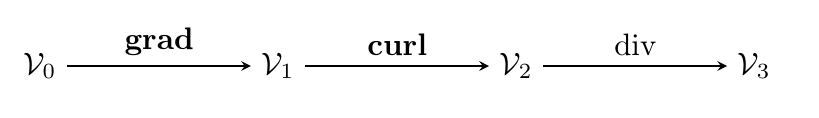
\includegraphics[width=.6\textwidth]{deRham3D.png}
\end{figure}
where $$\mathcal{V}_0 \subset H^1(\Omega),\ \mathcal{V}_1 \subset H(\textbf{curl};\Omega),\ \mathcal{V}_2 \subset H(\text{div};\Omega), \ \mathcal{V}_3 \subset L^2(\Omega)$$ are conforming subspaces. Each element of these spaces is uniquely determined by the degrees of freedom (DOFs), i.e. nodal values for $\mathcal{V}_0$, edge integrals for $\mathcal{V}_1$, face integrals for $\mathcal{V}_2$, and cell integrals for $\mathcal{V}_3$. In addition, a field can either belong to the primal or the dual complex.

In the code, fields are therefore initialized by a command of the form
\begin{center} \verb|DeRhamField<Grid, Space>|,\end{center}
where \verb|Grid| is either \verb|primal| or \verb|dual|, and \verb|Space| is either \verb|node|, \verb|edge|, \verb|face|, or \verb|cell|, in accordance to the DOFs.

In $2D$ (all fields only depend on $x$ and $y$) there are two de Rham sequences:

\begin{figure}[h]
\centering
	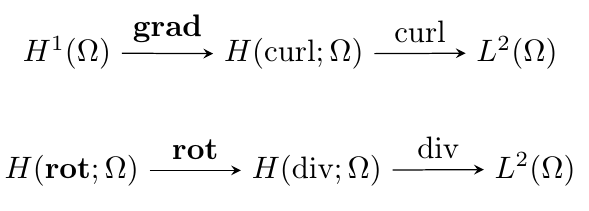
\includegraphics[width=.4\textwidth]{deRham2D.png}
\end{figure}
where the operators curl and $\mathbf{rot}$ are defined by
$$\text{curl} \begin{pmatrix} E_x \\ E_y \end{pmatrix} = \partial_x E_y - \partial_y E_x,$$ $$\mathbf{rot} (E_z) = \begin{pmatrix} \partial_y E_z \\ \partial_x E_z \end{pmatrix}.$$
In the code, these two sequences are embedded into the $3D$ complex by stacking them in the following way:
\begin{figure}[h]
\centering
	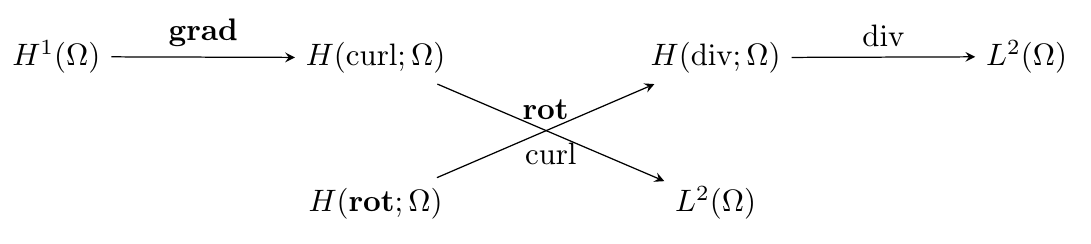
\includegraphics[width=.7\textwidth]{deRham2Dstacked.png}
\end{figure}
This means that in each $\mathcal{V}_i$ the fields have the same number of components as in $3D$, the spaces are given by
$$\mathcal{V}_0 = H^1(\Omega), \hspace{.5cm} \mathcal{V}_1 = \begin{pmatrix} H(\text{curl};\Omega)\\ H(\textbf{rot};\Omega) \end{pmatrix}, \hspace{.5cm} \mathcal{V}_2 = \begin{pmatrix} H(\text{div};\Omega)\\ L^2(\Omega) \end{pmatrix}, \hspace{.5cm} \mathcal{V}_3 = L^2(\Omega),$$
and the differential operators are
\begin{align*}
	\text{grad} (\varphi) &= \begin{pmatrix} \partial_x \varphi \\ \partial_y \varphi \\ 0 \end{pmatrix},\\
	\text{curl} \begin{pmatrix} E_x \\ E_y \\ E_z \end{pmatrix} &= \begin{pmatrix} \mathbf{rot}(E_z) \\ \text{curl} \begin{pmatrix} E_x \\ E_y \end{pmatrix} \end{pmatrix},\\
	\text{div} \begin{pmatrix} B_x \\ B_y \\ B_z \end{pmatrix} &= \partial_x B_x + \partial_y B_y.
\end{align*}
This way, any code written for $3D$ works without any modifications to the fields just the same in $2D$. A \verb|DeRhamField| defined on \verb|Space::edge| is still in $\mathcal{V}_1$, the only difference is that the third component will be node centered, since it belongs to $H(\mathbf{rot}; \Omega)$.

In $1D$ (all fields only depend on $x$) the implementation follows the same lines. There is only one de Rham sequence

\begin{figure}[h]
\centering
	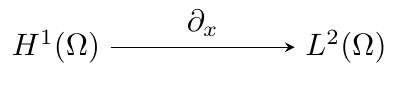
\includegraphics[width=.3\textwidth]{deRham1D.png}
\end{figure}
which is embedded into $3D$ complex in the following way:
\begin{figure}[h]
\centering
	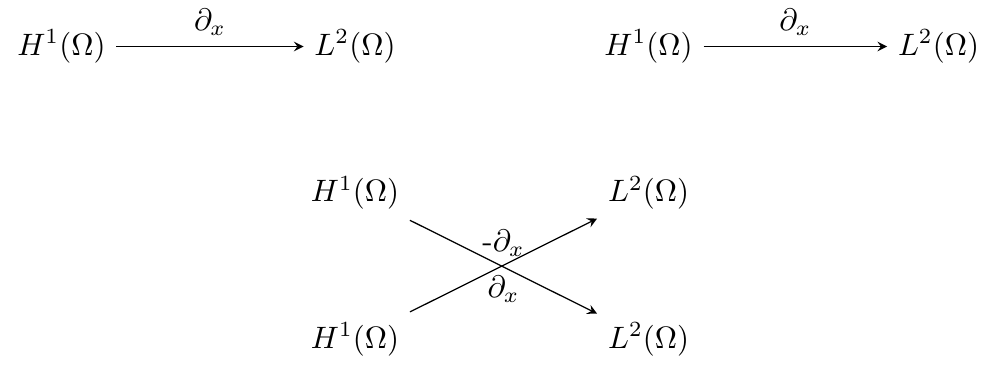
\includegraphics[width=.7\textwidth]{deRham1Dstacked.png}
\end{figure}

Again, the fields have the same number of components as in $3D$, the spaces are now given by
$$\mathcal{V}_0 = H^1(\Omega), \hspace{.5cm} \mathcal{V}_1 = \begin{pmatrix} L^2(\Omega)\\ H^1(\Omega) \\H^1(\Omega) \end{pmatrix}, \hspace{.5cm} \mathcal{V}_2 = \begin{pmatrix} H^1(\Omega)\\ L^2(\Omega) \\ L^2(\Omega) \end{pmatrix}, \hspace{.5cm} \mathcal{V}_3 = L^2(\Omega)$$
and the differential operators are
\begin{align*}
	\text{grad} (\varphi) &= \begin{pmatrix} \partial_x \varphi \\ 0 \\ 0 \end{pmatrix},\\
	\text{curl} \begin{pmatrix} E_x \\ E_y \\ E_z \end{pmatrix} &= \begin{pmatrix} 0 \\ -\partial_x E_z \\ \partial_x E_y \end{pmatrix},\\
	\text{div} \begin{pmatrix} B_x \\ B_y \\ B_z \end{pmatrix} &= \partial_x B_x.
\end{align*}
This way, any code written for $3D$ works without any modifications to the fields just the same in $1D$. A \verb|DeRhamField| defined on \verb|Space::edge| is still in $\mathcal{V}_1$, the only difference is that the second and third component will be node centered, since they belong to $H^1(\Omega)$.
\end{document}